\documentclass{fkpset}

% \newgeometry{bmargin=1in, tmargin=1.25in, lmargin=.75in, rmargin=.75in}
% \fancyhfoffset[R]{.05cm}

\name{Forest Kobayashi}
\class{Math 147}
\duedate{03/27/2019}
\assignment{HW 6 Solutions}

\chead{HW 6 Sample Solutions}
\rhead{Math 147 -- Spring, 2019}

\lfoot{Wednesday, March 27th 2019}

\problems{5.29, 5.32, 6.6, 6.11, 6.18}

\usepackage{hyperref}

\usetikzlibrary{hobby}

\newcommand{\tstd}{\ensuremath \ms T_{\rm std}}
\newcommand{\tprod}{\ensuremath \ms T_{\rm prod}}

\begin{document}
\pagestyle{plain}
\pagestyle{fancy}
  % \vspace{-2.9cm}
  \pointstable{}

  \vspace{1cm}

% --------------------------- Problem 1 ---------------------------- %
  \begin{problem}[5.29 (The Normality Lemma)]
    Let $A$ and $B$ be subsets of a topological space $X$ and let
    $\set{U_i}_{i \in \NN}$ and $\set{V_i}_{i \in \NN}$ be two
    collections of open sets such that
    \begin{enumerate}[label=(\arabic*)]
      \item $A \subset \bigcup_{i \in \NN} U_i$
      \item $B \subset \bigcup_{i \in \NN} V_i$
      \item For each $i \in \NN$, $\ol{U_i} \cap B = \varnothing$ and
        $\ol{V_i} \cap A = \varnothing$.
    \end{enumerate}
    Then there exist open sets $U$ and $V$ such that $A \subset U$, $B
    \subset V$, and $U \cap V = \varnothing$.
  \end{problem}
  \begin{leftbar}
    Before a solution, I'll give some intuition on how we might arrive
    at the candidate $U,V$ that work.

    Let's think about what we're given. We have $\set{U_i}_{i \in
      \NN}$, and $\set{V_i}_{i \in \NN}$ as defined above, and we want
    to use them to construct $U,V$ satisfying the given constraints.
    It seems like it'd be straightforward to satisfy $A \subset U$, $B
    \subset V$ --- they look like they'll probably fall directly out
    of the conditions. $U \cap V = \varnothing$ is harder, since we're
    given no direct information about $U_i \cap V_j$. Hence, we'll
    pick the following as our general approach:
    \begin{enumerate}[label=(\arabic*)]
      \item Think about what
        \[
          \tilde U = \bigcup_{i \in \NN} U_i \qquad\qquad \tilde V =
          \bigcup_{i \in \NN} V_i
        \]
        look like. In particular, we'll focus on the conditions that
        break/make $\tilde U$ and $\tilde V$ \emph{not} work as
        choices of $U,V$. Then,
      \item We'll see if we can find a clever way to remove the parts
        of $U_i$ and $V_i$ that cause problems. If all goes right,
        we'll find sequences $\set{U'_i}_{i\in\NN}$,
        $\set{V'_i}_{i\in\NN}$ whose terms can be unioned to get
        $U,V$.
    \end{enumerate}
    Depict our two sets $A,B$ as
    follows:
    \begin{center}
      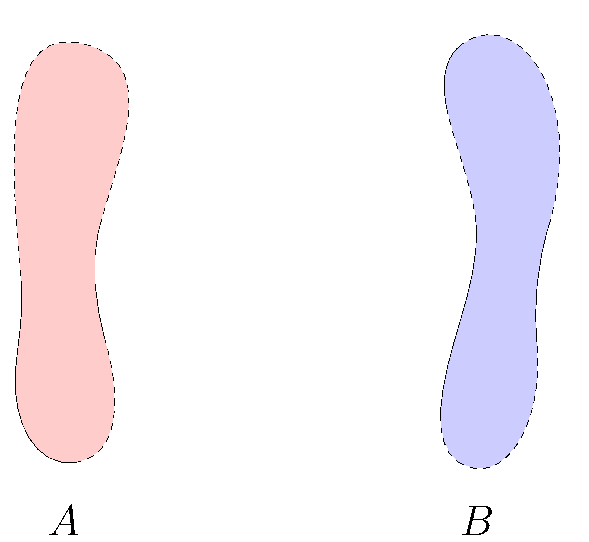
\includegraphics[keepaspectratio,width=6cm]{figures/5-29-AB}
    \end{center}
    To make the TikZ easier, I'll draw our covers with boxes --- but
    note, in general they could be blobby. Anyways, we now draw
    $U_1, V_1$:
    \begin{center}
      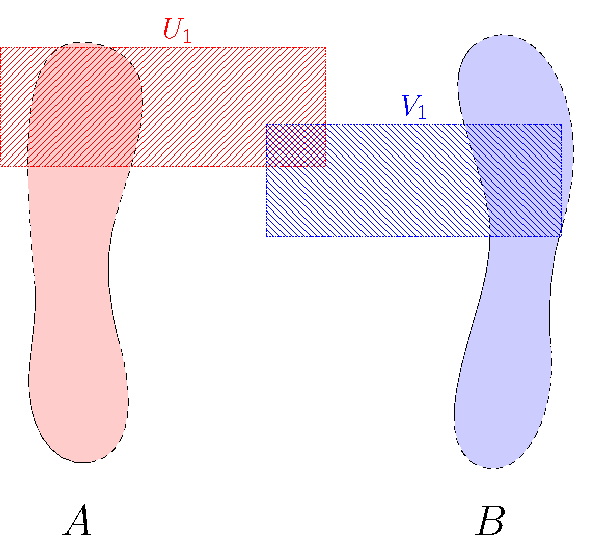
\includegraphics[keepaspectratio,width=6cm]{figures/5-29-n=1}
    \end{center}
    We need to be sure that in our construction of $U$, we don't
    include any of the $V_i$. We want to use the $U_i$, but as we can
    see, they might intersect the $V_i$. The fix? Remove the parts
    that cause problems. We define
    \begin{align*}
      U_1'
      &= U_1 - \ol{V_1}
      &
      V_1'
      &= V_1 - \ol{U_1}
    \end{align*}
    which yields
    \begin{center}
      \includegraphics[keepaspectratio, width=6cm]{figures/5-29-n=1-primes}
    \end{center}
    Now, we consider $n=2$:
    \begin{center}
      \includegraphics[keepaspectratio, width=6cm]{figures/5-29-n=2}
    \end{center}
    We already know how to rectify $U_1, V_1$:
    \begin{center}
      \includegraphics[keepaspectratio, width=6cm]{figures/5-29-n=2-prime1}
    \end{center}
    but we still have a problem now. Our addition of $U_2, V_2$ is
    complicating the situation! Namely, we have $U_2 \cap V'_1 \neq
    \varnothing$, $U_2 \cap V_2 \neq \varnothing$.\footnote{Note we
      could also have the analogous for $V_2 \cap U'_1$ if $V_2$ were
      a bit larger.} We \emph{don't} want to go back and edit our
    definitions for $U'_1, V'_1$ --- if we were to take this approach,
    we'd need to proceed similarly for $n=2$, $n=3$, etc.\ until
    eventually $U'_1 = U_1 - \bigcup_{i\in\NN} \ol{V_i}$, which could
    cause some problems.

    Instead, we'll modify $U_2$ and $V_2$, leaving $U'_1$ and $V'_1$
    untouched. Hence, we let
    \[
      U'_2 = U_2 - (\ol{V_1} \cup \ol{V_2}) \qquad\qquad
      V'_2 = V_2 - (\ol{U_1} \cup \ol{U_2})
    \]
    which gives us
    \begin{center}
      \includegraphics[keepaspectratio, width=6cm]{figures/5-29-n=2-prime2}
    \end{center}
    From which we can see $(U'_1 \cup U'_2) \cap (V'_1 \cup V'_2) \neq
    \varnothing.$ Thus, we conjecture that in the general case,
    \[
      U'_n = U_n - \bigcup_{i=1}^n \ol{V_i} \qquad\qquad V'_n = V_n -
      \bigcup_{i=1}^n \ol{U_i}
    \]
    will work.
  \end{leftbar}
  \begin{solution}

  \end{solution}
  \clearpage

% --------------------------- Problem 2 ---------------------------- %

  \begin{problem}[5.32]
    Suppose a space $X$ is regular and has a countable basis. Then $X$
    is normal.
  \end{problem}
  \begin{solution}
    Let $A,B$ be disjoint closed sets.
  \end{solution}
  \clearpage

% --------------------------- Problem 3 ---------------------------- %
  \begin{problem}[6.6]
    The space $2^\RR$ is separable.
  \end{problem}
  \begin{solution}
    % We first find a candidate countable dense subset.
    \begin{leftbar}
      Let
      \[
        S = \set{\bigcup_{i=1}^n (p_i, q_i) \MID n \in \NN,\
          \text{and}\ p_i, q_i \in \QQ \text{ for each $i$}}.
      \]
      First, note that the set comprehension above yields at most
      countably many elements (the set of all finite subsets of a
      countable set is countable). Hence, $S$ is at most countable.

      Now, note that $S$ has a countably infinite subset:
      \[
        S' = \set{(0,q) \MID q \in \QQ} \subset S.
      \]
      Thus $S$ is at least countably infinite as well. So $\abs{S} =
      \abs{\NN}$. \cmark
    \end{leftbar}
    Now, let
    \[
      \mc F = \set[bigg]{f : \RR \to \set{0,1} \MID f\fpre[\set{1}]
        \in S}.
    \]
    where $f\fpre[\set{1}]$ denotes the preimage of $\set{1}$. Also
    let

    % We claim $\ol{\mc F} = 2^\RR$.

    Let $U \in \ms T_{2^\RR}$ be arbitrary. Then by definition of the
    product topology,
    \[
      U = \prod_{\xi\in \RR} X_\xi
    \]
    where $X_\xi$ is open in $\set{0,1}$ under the discrete topology,
    and $X_\xi = \set{0,1}$ for all but finitely many $\xi$. Let
    $\set{X_{\xi_i}}_{i=1}^n$ be this finite collection of $X_\xi$,
    and for each $i$, let $Y_i = $
  \end{solution}
  \clearpage

% --------------------------- Problem 4 ---------------------------- %
  \begin{problem}[6.11]
    Every uncountable set in a 2\textsuperscript{nd} countable space
    has a limit point.
  \end{problem}
  \begin{solution}
    Let $(X, \ms T)$ be a 2\textsuperscript{nd} countable space with
    countable basis $\ms B$, and let $A \subset X$ be uncountable.

    Let $a \in A$. Suppose, to obtain a contradiction, that $A$ has no
    limit points. Then $a$ is an isolated point of $A$, and by Theorem
    3.10, there exists $U_a \in \ms T \st U_a \cap A = \set{a}$. Then
    by definition of a basis, there exists $B_a \in \ms B$ such that
    \[
      a \in B_a \subset U_a,
    \]
    and hence
    \[
      B_a \cap A = \set{a}
    \]
    as well. It follows that $\ms B' = \set{B_a}_{a \in A}$ is an
    uncountable subset of $\ms B$, a contradiction.

    Thus, $A$ has a limit point.
  \end{solution}
  \clearpage

% --------------------------- Problem 5 ---------------------------- %
  \begin{problem}[6.18]
    Suppose $x$ is a limit point of the set $A$ in a
    1\textsuperscript{st} countable space $X$. Then there is a
    sequence of points $\set{a_i}_{i \in \NN}$ that converges to $x$.
  \end{problem}
  \begin{solution}
  \end{solution}

\end{document}